% This is samplepaper.tex, a sample chapter demonstrating the
% LLNCS macro package for Springer Computer Science proceedings;
% Version 2.20 of 2017/10/04
%
\documentclass[runningheads]{llncs}
%
\usepackage{graphicx}
\usepackage{epstopdf}
% Used for displaying a sample figure. If possible, figure files should
% be included in EPS format.
%
% If you use the hyperref package, please uncomment the following line
% to display URLs in blue roman font according to Springer's eBook style:
% \renewcommand\UrlFont{\color{blue}\rmfamily}

\begin{document}
%
\title{Processing of medical data by artificial intelligence for medical diagnosis support}
%
%\titlerunning{Abbreviated paper title}
% If the paper title is too long for the running head, you can set
% an abbreviated paper title here
%
\author{Matej Horniak\thanks{Bachelor study programme in field: Informatics.
Supervisor: doc. Ing. Vanda Benešová, PhD., Faculty of Informatics
% , Institute of Informatics, Information Systems and Software Engineering
and Information Technologies STU in Bratislava }
% \orcidID{0000-1111-2222-3333}
}


% \authorrunning{F. Author et al.}
% First names are abbreviated in the running head.
% If there are more than two authors, 'et al.' is used.
%
\institute{Slovak University of Technology in Bratislava \\
Faculty of Informatics and Information Technologies \\
Ilkovičova 2, 842 16 Bratislava, Slovakia \\
\email{xhorniakm@stuba.sk}}
%
\maketitle              % typeset the header of the contribution
%
\begin{abstract}
The highest number of deaths caused by cancer is caused by breast cancer, which is the most frequent type of cancer diagnosed for women. One of the most reliable methods to confirm this diagnosis is a biopsy, which is a very difficult and lengthy process because it consists of a large amount of microscopic(histological) data. Nowadays, we are able to see the rise of automatic data processing using computer vision and deep learning. This automation provides us with a lot of benefits, such as efficient and faster data processing or more accuracy. 

V tejto praci sa zameriavame na klasifikaciu histologickych dat pomocou hlbokych neuronovych sieti a to konvolucnych neuronovych sieti. Hlavnou myslienkou je porovnanie roznych principov pre vytvaranie filtrov v prvych vsrtvach neuronovej siete. Porovnavame automaticke vytvaranie filtrov a manualne. Za automaticke vytvaranie fitlrov sme zvolili klasicky backpropagation, autoencoder a transfer learning. A pre manualne vytvaranie filtrov sme zvolili gaborove filtre.  
\keywords{Artificial intelligence \and Machine learning  \and Medical data \and Gabor filters \and Transfer learning \and Autoencoder \and Backpropagation}
\end{abstract}
%
%
%
\section{Introduction}
Najväčší počet úmrtí na rakovinu je spôsobený rakovinou prsníka, u žien je to najfrekventovanejšie diagnostikovaná rakovina. Podľa celosvetových štatistických meraní postihuje hlavne ženy vo veku okolo 50 rokov. Táto rakovina sa môže vyskytnúť aj u mužov. Vzniká nadmerným nekontrolovateľným delením buniek mliekovodov a lalôčikov. 

Spracovanie histologických dát je jednou z najnáročnejších techník diagnózy rakoviny. Kvôli tejto skutočnosti sa vykonáva až ako posledná, aj keď jej výsledky sú najpresnejšie. Vďaka tomuto vyšetreniu môžeme s vysokou pravdepodobnosťou potvrdiť správnosť diagnózy. Histologické vyšetrenie spočíva v tom, že doktor vykoná biopsiu napadnutej časti tela, odoberie vzorku z malej časti tkaniva, ktorú odošle na laboratórne spracovanie. V laboratóriu sa uloží vzorka pod mikroskop, kde sa po jej niekoľkonásobnom zväčšení  preskúma prítomnosť rakoviny v každej bunke. 

Táto časť vyšetrenia býva zväčša rutinná a nie je potrebná interakcia s pacientom, preto túto časť dokážeme zautomatizovať. A to vďaka odvetviu počítačovej vedy, umelej inteligencie.

Vďaka nástupu hlbokého učenia neurónových sietí je možné zlepšiť presnosť  výsledkov spracovávaných dát a množstvo dát, ktoré dokážeme spracovávať. Jedinou nevýhodou tejto metódy (spracovania diagnostických vyšetrení pomocou neurónových sietí)  je, že pre svoju existenciu a presnejšie určenie výsledkov potrebuje obrovské množstvo dát na trénovanie. 

V práci sa zameriavame hlavne na použitie rôznych typov filtrov  konvolučných neurónových sietí. Porovnáme princípy tvorenia filtrov manuálne a automaticky, filtre, ktoré si neurónová sieť vytvára sama. Tieto filtre sa zameriavaju na detekciu rakoviny v histologických dátach.
\section{Related Work}

\subsection{Publikácia Transfer learning based deep CNN for segmentation and detection of mitoses in breast cancer histopathological images \cite{Transferlearningbaseddeep}}

V práci o segmentácii a detekovaní mitózy v rakovine prsníka sa používajú dve konvolučné neurónové siete. Tieto siete sú navzájom prepojené. Segmentačná používa Transfer learning, kde model, od ktorého preberá váhy, je ImageNet sieť, ktorá obsahuje približne 1000 kategórií na rozpoznávanie prirodzených farebných obrázkov.

Prvá konvolučná neurónová sieť sa používa na segmentáciu mitóz. Súbory (patch), ktoré sú extrahované,  slúžia ako vstup do druhej, ktorá je hybridno konvolučná a to tak, že kombinuje Weight Transfer a custom vrstvu pre finálnu klasifikáciu. Vysledky klasifikácie sú rozdelené do dvoch kategórií, na "mitózy” a "nie mitózy”. Vďaka týmto dvom fázam, učením 2 neurónových sietí, sa zmenšuje efekt nerovnováhy obsadenosti jednotlivých kategórií v histologických dátach.

Dáta z datasetu pre TUPAC16 získali presnosť 66,7\%, pričom pokiaľ použili pri validácií dáta aj z MITOS12 a MITOS14, získali sme presnosť 65,1\%. No pokiaľ bol model trénovaný od začiatku na všetkých dátach, jednotlivé presnosti sa zmenšili, teda pokiaľ validačný dataset bol TUPAC16 a presnosť bola 65\%. Validačný dataset pozostával z oboch zdrojov, presnosť bola 63,6\% a pri MITOS12 a MITOS14 bola 59,7\%. Tieto výsledky sú zhrnuté v tabuľke \ref{fig:SegaDetNN} 

\begin{figure}[h!]
\begin{centering}
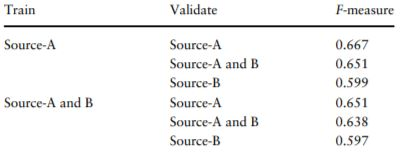
\includegraphics[width=10cm]{253_2.JPG}
\par\end{centering}
\caption{Výsledky pre segmentáčnú a detekčnú neurónovú sieť (zdroj A je TUPAC16, zdroj B je MITOS12 a MITOS14). \label{fig:SegaDetNN}\cite{Transferlearningbaseddeep}}
\end{figure}

\subsection{Publikácia s názvom Classification of  breast cancer histology images using Convolutional Neural Networks \cite{ClassificationBreastCancer}}

Publikácia bola zverejnená v roku 2017 talianskou univerzitou.  V  tejto práci sa využívajú konvolučné neurónové siete pre klasifikáciu rakoviny prsníka. Obrazy sa rozdeľujú do 4 kategórií a to normálne tkanivo, počiatočné lézie, in situ karcinóm a invazívny karcinóm. V práci sa používajú konvolučné neurónové siete samostatne a aj s pomocou Support Vector machine klasifikácie. Konvolučná neurónová sieť je navrhnutá pre analýzu histologických obrázkov rakoviny prsníka H\&E. Okrem toho je architektúra konvolučnej neurónovej siete navrhnutá tak, aby dokázala získať informácie z viacerých histologických stupňov vrátane nuklidu, usporiadania nuklidu  a celkového usporiadania štruktúry. Zohľadnením  konvolučnej neurónovej siete sa môže použiť aj na klasickú klasifikačnú úlohu celoobrazových histologických obrazov.

Patch-wise technika dosiahla presnosť a citlivosť zobrazenú v tabuľke \ref{fig:vysledkyPatch-Wise}. Celková presnosť je 66,7\% pre konvolučnú neurónovú sieť a pre konvolučnú neurónovú sieť s podporou support vector machine algoritmu to je 65\%. Presnosť systému je nízka, pre rozšírený dataset kvôli zníženej časovej náročnosti. Celková presnosť sa zvýši, pokiaľ sa zmení počet kategórií zo štyroch na dve. Teda ak triedy normálne tkanivo a začiatočné lézie, in situ a invazívny karcinóm spojíme,  dosiahneme až 80\% presnosť. \cite{ClassificationBreastCancer}

\begin{figure}[h!]
\begin{centering}
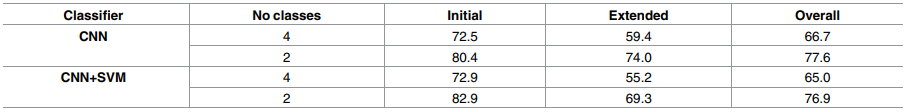
\includegraphics[width=15cm]{252_5.png}
\par\end{centering}
\caption{Výsledky patch-wise techniky konvolučnej neurónovej siete. \label{fig:vysledkyPatch-Wise}\cite{ClassificationBreastCancer}}
\end{figure}

\section{Our work}

Nasu pracu sme implementovali v jazyku python a hlavnu cast pomocou kniznice Keras a Tensorflow.
Vysledky su ziskavane na Datasete PatchCamelyon (PCAM), ktory je rozdeleny na 262144 obrazkov pre trenovanie, 32768 obrazkov pre validaciu a 32768 obrazkov pre testovanie. 
Tieto obrazky su v rozmeroch 96x96x3, pricom na obrazkoch sa nachadzaju fotky histologickych dat roznych organov.\cite{pcam} 
Pre tento dataset najlepsie vysledky dosiahla architektura unet, ktora mala presnost okolo 78-82\%. 
Ostatne architektury, ktore sme vyskusali su VGG 16, ktora dosiahla 50\% presnost (accuracy). dalej to bol ResNet s hlbkou 8, ktora dosiahla 67.2\%. 
Vyskusali sme este aj neuronove siete, ktore boli zlozene maximalne z 5 konvolucnych vrstiev, pricom vysledky sa nachadzaju v tabulke cislo  \ref{tab2}. 
Tieto neuronove siete po Flatten vrstve 2 Dense vrstvy s 128 neuronmi. 

\begin{table}
\caption{Vysledky pre CNN s max 5 vrstvami.}\label{tab2}
\begin{tabular}{|l|l|l|}
\hline
Pocet vrstiev & velkost filtrov & Presnost \\
\hline
3 conv & 2x3 velkost filtra 1x5 velkost filtra & 74,9\% \\
3 conv & 2x3 velkost filtra 1x5 velkost filtra & 73\% \\
3 conv without dropout & 2x3 velkost filtra 1x5 velkost filtra & 72,29\% \\
5 conv & 2x5 velkost filtra & 63\% \\
2 conv & 2x3 velkost filtra & 74,6\% \\
\hline
\end{tabular}
\end{table}

Takze architektura, ktora najlepsie riesila danu klasifikaciu bola Unet architektura. 
Ta obsahuje 9 convolutional vrstiev. Tuto architekturu sme zobrali ako zaklad pre dalsie preskumavanie a porovnavanie. 
Nasledne modely pozostavaju z unet architektury pred ktoru vlozime vrstvu, ktora vzdy meni principy tvorenia fitlrov. 
A to bud si filtre tvori (uci) sama alebo su zadefinovane a stracaju schopnost ucit sa. 
Pouzili sme zatial tri typy filtrov na prvej vrstve a to 
\begin{enumerate}
\item Backpropagation, ktore bolo vytvorene ako obycajna convolucna vrstva pre Unet architekturu, a ta sklada z Conv2D, BatchNormalization, Activation function a druha skryte vrstva Conv2D, BatchNormalization, Activation function. Po tejto kombinacii pridame MaxPooling2D s velkostou 2 a dropout vrstvu pre zmiernenie pretrenovania.
\item Autoencoder, ktore je zlozene z Conv2D, Droupout, Conv2D, MaxPooling2D s velkostou 2 a Conv2D, Droupout, Conv2D, pricom posledna vrstva sa zlucuje pomcoou Concatenate a UpSampling2D s velkostou 2.
\item Gabor filters, tuto vrstvu si vytvorime s tym, ze jej zakazeme naucit sa vahy. Nasledne pomocou kniznice opencv vytvorime gaborove filtre a vlozime do Conv2D vrstvy ako vahy (weights).
\end{enumerate}
Pricom vo vsetkych pripadoch pouzivame aktivacnu funkciu relu a pridavame padding typu "same". 
Pre jednotlive typy sme dostali nasledovne vysledky pri obmedzenych parametrov Backpropagation, obsahoval 16 filtrov s velkostou 16 a presnostou 80\%. 
Autoencoder dosiahol 80,524\% presnost pri 32 filtroch o velkosti 3 a pre Gaborove fitltre to 80,47\% prenost kde vlozenych bolo 32 filtrov o velkosti 7. 

\section{Conclusion and future work}

Klasifikacia nad histologickymi datami je velmi zlozity proces, ci uz sa to tyka z obmedzeneho mnozstva dat pre trenovanie, zlozitostou rozoznavania, kde aj clovek ma velmi velke problemy najst bunky rakoviny, alebo casovou narocnostou trenovania. 
modely a porovnanie, ktore sme vytvorili a vyskusali, nam dali rozne vysledky a to. 
Pri architekture aj male modely, tvorene malym poctom vrstiev, su dobre efektivne a niekedy viac ako zlozite architektury. 
Co sa tyka jednotlivych typov filtrov v prvych vrstvach, tieto nam zatial dali podobne vysledky, a rozdieli boli len v desatinnych cislach. 

Preto chceme tieto porovnania rozsirit a tym zistit viacere vyhody nevyhody jednotlivych principov, pricom pridame princip, ktory pouzili iny ako jedine riesenie pre klasifikaciu nad histologickymi datami.
A to transfer learnning, kde vyuzivame filtre, ktore sa siet uz naucila aj ked nie na nasich datach.
Nasledne budeme sa snazit zistit, ktory princip je najlepsi, ci uz je to obycajny backpropagation, autoencoder, gaborove fitlre alebo transfer learning. 
Porovnavanie bude pozostavat minimalne z 9 neuronovych sieti z kazdeho principy, pricom pri prvych troch budeme menit parametre prvych vrstiev a to pocet filtrov a velkost jednotlivych filtrov. 
Jednotlive hodnoty pre vsetky tri principy, budeme volit pocet filtrov, medzi 16, 32 a 64. A pri backpropagation a autoencoderu budeme menit velkost filtrov, medzi 3, 5 a 7. 
Pri Gaborovych filtrov budeme pouzivat velkosti 5, 7 a 9. Pri transfer learningu je komplikovajsie upravovanie filtrov kedze pouzivame uz vytvorene filtre a tie nechceme menit.
Takze budeme menit pocet filtrov kolko sa moze znova naucit siet, a mozno popridanie nie konvolucnych vrstiev. 
Celkove vysledky rozsirime o viacere metriky, teda nie len accuracy ale aj precision, recall, f1 score a true positives. 
Vysledky berieme len z testovacej mnoziny, teda data, ktore siet nikdy predtym nevidela. 
% Nasledne najlepsie vysledky porovname na druhom datasete a to ECDP \cite{ECDP}, ktory obsahuje histologicke data rakoviny prsnika, okolo 360 obrazkov v MIRAX formate.

%
% ---- Bibliography ----
%
% BibTeX users should specify bibliography style 'splncs04'.
% References will then be sorted and formatted in the correct style.
%
\bibliographystyle{splncs04}
\bibliography{mybibliography}

\begin{thebibliography}{8}


\bibitem{goodfellow}
Goodfellow, I. and Bengio, Y. and Courville, A.: Deep Learning, MIT Press, 167-523 (2016)

\bibitem{NovelDeepLearning}
Khan. S. U. and Islam, N. and Jan, Zahoor and Din, I. U. and Rodrigues, J. J. P. C: A novel deep learning based framework for the detection and classification of breast cancer using transfer learning. Pattern Recognition Letters

\bibitem{ClassificationBreastCancer}
Ara{\'u}jo, T. and Aresta, G. and Castro, E, and Rouco, J. and Aguiar, P. and Eloy, c. and Pol{\'o}nia, A. and Campilho, A.: Classification of breast cancer histology images using convolutional neural networks. PloS one, (2017)

\bibitem{Transferlearningbaseddeep}
Wahab, N. and Khan, A. and Lee, Y. S.: Transfer learning based deep CNN for segmentation and detection of mitoses in breast cancer histopathological images, Microscopy, 216-233 (2019)

\bibitem{pcam}
Veeling, Bastiaan S and Linmans, Jasper and Winkens, Jim and Cohen, Taco and Welling, Max: Rotation Equivariant {CNNs} for Digital Pathology, (2018)

% \bibitem{ECDP}
% Silva, AM. and Santos, M.: ECDP2020: Stanford University, Computer Science Department, 156 Gates Building 1A, Stanford CA 94305, (2019)

% \bibitem{ref_article1}
% Author, F.: Article title. Journal \textbf{2}(5), 99--110 (2016)

% \bibitem{ref_lncs1}
% Author, F., Author, S.: Title of a proceedings paper. In: Editor,
% F., Editor, S. (eds.) CONFERENCE 2016, LNCS, vol. 9999, pp. 1--13.
% Springer, Heidelberg (2016). \doi{10.10007/1234567890}

% \bibitem{ref_book1}
% Author, F., Author, S., Author, T.: Book title. 2nd edn. Publisher,
% Location (1999)

% \bibitem{ref_proc1}
% Author, A.-B.: Contribution title. In: 9th International Proceedings
% on Proceedings, pp. 1--2. Publisher, Location (2010)

% \bibitem{ref_url1}
% LNCS Homepage, \url{http://www.springer.com/lncs}. Last accessed 4
% Oct 2017
\end{thebibliography}
\end{document}



% \subsection{A Subsection Sample}
% Please note that the first paragraph of a section or subsection is
% not indented. The first paragraph that follows a table, figure,
% equation etc. does not need an indent, either.

% Subsequent paragraphs, however, are indented.

% \subsubsection{Sample Heading (Third Level)} Only two levels of
% headings should be numbered. Lower level headings remain unnumbered;
% they are formatted as run-in headings.

% \paragraph{Sample Heading (Fourth Level)}
% The contribution should contain no more than four levels of
% headings. Table~\ref{tab1} gives a summary of all heading levels.

% \begin{table}
% \caption{Table captions should be placed above the
% tables.}\label{tab1}
% \begin{tabular}{|l|l|l|}
% \hline
% Heading level &  Example & Font size and style\\
% \hline
% Title (centered) &  {\Large\bfseries Lecture Notes} & 14 point, bold\\
% 1st-level heading &  {\large\bfseries 1 Introduction} & 12 point, bold\\
% 2nd-level heading & {\bfseries 2.1 Printing Area} & 10 point, bold\\
% 3rd-level heading & {\bfseries Run-in Heading in Bold.} Text follows & 10 point, bold\\
% 4th-level heading & {\itshape Lowest Level Heading.} Text follows & 10 point, italic\\
% \hline
% \end{tabular}
% \end{table}


% \noindent Displayed equations are centered and set on a separate
% line.
% \begin{equation}
% x + y = z
% \end{equation}
% Please try to avoid rasterized images for line-art diagrams and
% schemas. Whenever possible, use vector graphics instead (see
% Fig.~\ref{fig1}).

% \begin{figure}
% \includegraphics[width=\textwidth]{fig1.eps}
% \caption{A figure caption is always placed below the illustration.
% Please note that short captions are centered, while long ones are
% justified by the macro package automatically.} \label{fig1}
% \end{figure}

% \begin{theorem}
% This is a sample theorem. The run-in heading is set in bold, while
% the following text appears in italics. Definitions, lemmas,
% propositions, and corollaries are styled the same way.
% \end{theorem}
% %
% % the environments 'definition', 'lemma', 'proposition', 'corollary',
% % 'remark', and 'example' are defined in the LLNCS documentclass as well.
% %
% \begin{proof}
% Proofs, examples, and remarks have the initial word in italics,
% while the following text appears in normal font.
% \end{proof}
% For citations of references, we prefer the use of square brackets
% and consecutive numbers. Citations using labels or the author/year
% convention are also acceptable. The following bibliography provides
% a sample reference list with entries for journal
% articles~\cite{ref_article1}, an LNCS chapter~\cite{ref_lncs1}, a
% book~\cite{ref_book1}, proceedings without editors~\cite{ref_proc1},
% and a homepage~\cite{ref_url1}. Multiple citations are grouped
% \cite{ref_article1,ref_lncs1,ref_book1},
% \cite{ref_article1,ref_book1,ref_proc1,ref_url1}.